\documentclass{beamer}
\setbeamertemplate{section in toc}[sections numbered]		% Numbered sections in the table of contents
%\usepackage{hyperref}
%\usepackage{multimedia}										% Animations on the slides
%\usepackage{media9}
\usepackage{animate}
\usetheme[progressbar=frametitle, block=fill]{metropolis} % Use metropolis theme
%\usecolortheme{seahorse}
%\usetheme{Verona} % Use verona theme

\usepackage{blindtext}			% Generates dummy text
\usepackage{url}				% Adding url's
\usepackage{physics}			% Some physics' notations
\usepackage{xcolor}				% Highlights text
\usepackage{graphicx}			% For Graphics	
\graphicspath{{../Plots/}}		% Path of the images
\usepackage{copyrightbox}		% Copyright
%\usepackage[style=verbose,backend=biber]{biblatex}
%\addbibresource{../Blibiography.bib}

\makeatletter
\renewcommand{\CRB@setcopyrightfont}{\tiny}

\definecolor{mLightGreen}{HTML}{14B03D}


\title{Codecademy Capstone Project\\Netflix Stock Profile}
%\subtitle{}
\author{Pedro Henrique Barboza Rossetto}
\date{\today}
\institute{}
\metroset{sectionpage=none}


\begin{document}
\maketitle

\begin{frame}
	\tableofcontents
\end{frame}

\section{Netflix Stock by Quarter}
\begin{frame}{Netflix Quarterly Stock Price}
	\begin{figure}
		\centering
		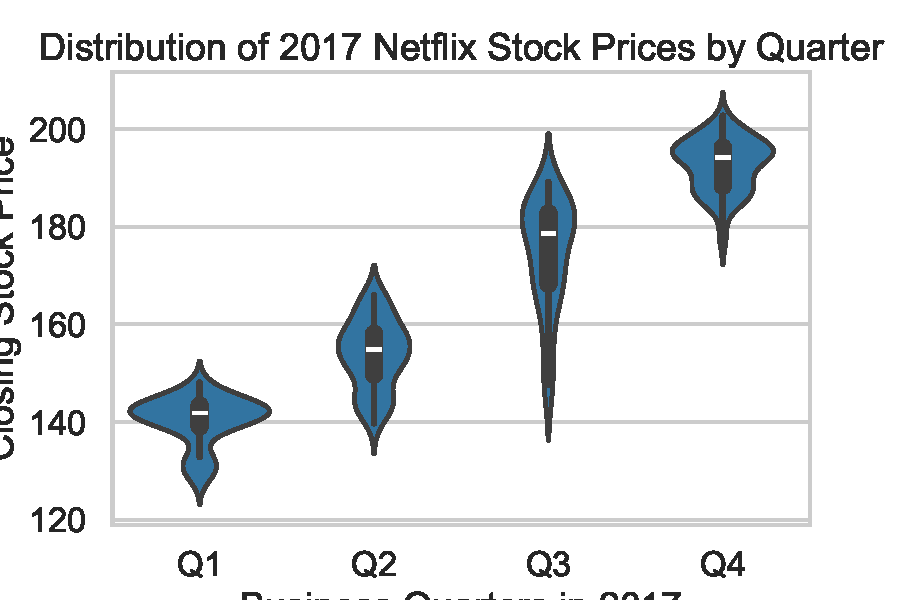
\includegraphics[width=\textwidth]{1-violin_plot_netflix_stock_by_quarter.pdf}
	\end{figure}
\end{frame}

\begin{frame}{Netflix Quarterly Stock Price - Description and Analysis}
	\begin{itemize}
		\item The average price of Netflix stock has gone up for every quarter of 2017.
		\item The minimum stock price was $\$ 129.46$ and the maximum was $\$ 202.68$.
		\item The third quarter showed the largest price fluctuation.
	\end{itemize}
\end{frame}

\section{Estimated and Actual Earnings}
\begin{frame}{Estimated and Actual Earnings}
	\begin{columns}[c]
		\begin{column}{0.6\textwidth}
			\begin{figure}
				\centering
				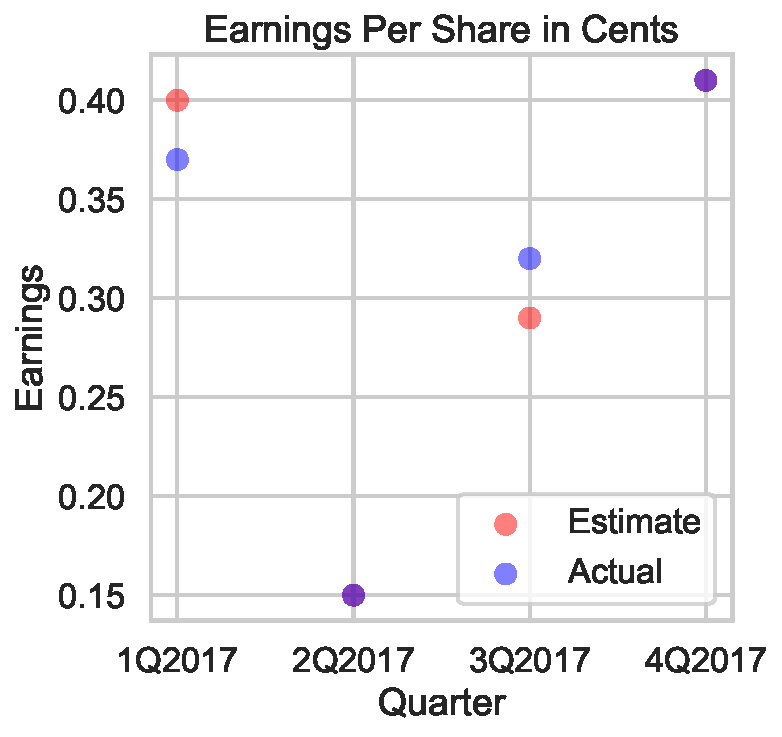
\includegraphics[width=\textwidth]{2-estimitate_and_actual_earnings.pdf}
			\end{figure}
		\end{column}
		\begin{column}{0.5\textwidth}
			\begin{itemize}
				\item The estimates by quarter price followed well the actual earnings.
				\item In the second and fourth quarters the estimates and the actual earnings were the same.
			\end{itemize}
		\end{column}
	\end{columns}
\end{frame}

\section{Netflix Earnings and Revenue}
\begin{frame}{Netflix Earnings and Revenue}
	\begin{figure}
		\centering
		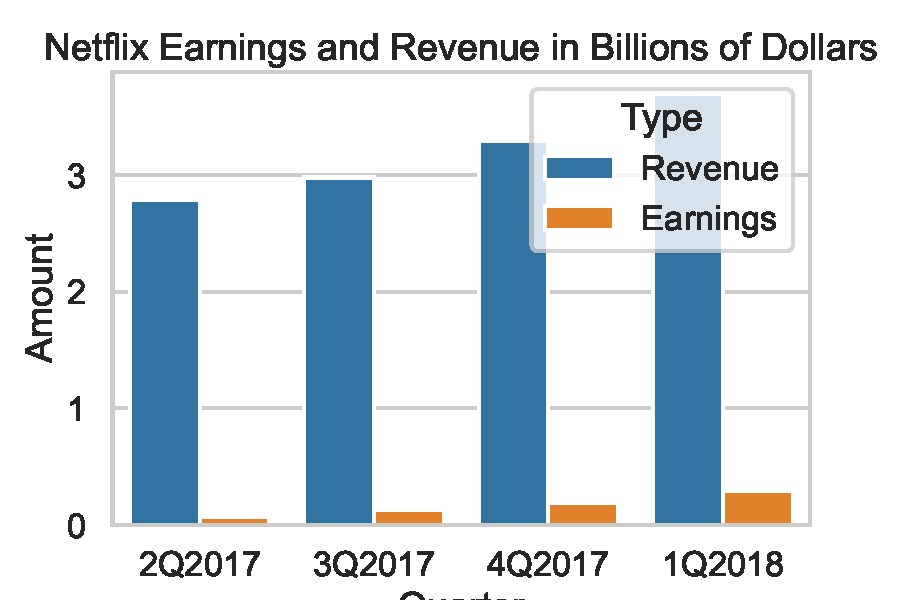
\includegraphics[width=\textwidth]{3-netflix_earnings_and_revenue.pdf}
	\end{figure}
\end{frame}

\begin{frame}{Netflix Earnings and Revenue - Description and Analysis}
	\begin{itemize}
		\item Both earnings and revenue grew throughout the quarters of 2017.
		\item The earnings are roughly $5\%$ of the total revenue.
	\end{itemize}
\end{frame}

\section{Netflix on the Stock Market Context}
\begin{frame}{Netflix on the Stock Market Context}
	\begin{figure}
		\centering
		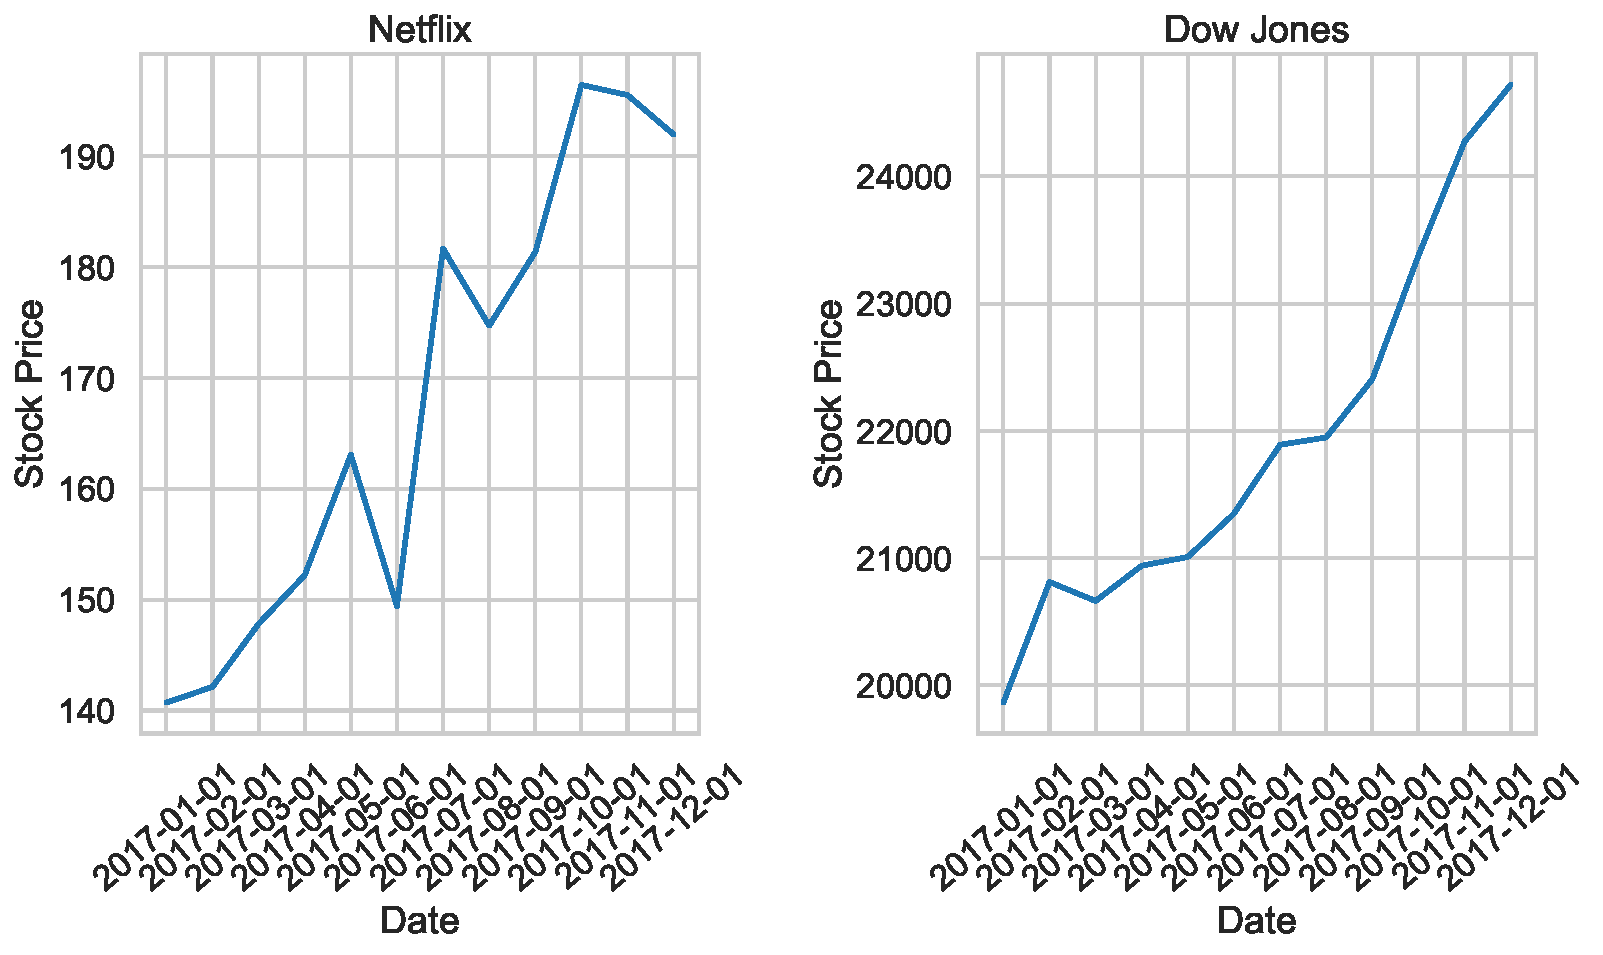
\includegraphics[width=\textwidth]{4-netflix_and_dow_jones.pdf}
	\end{figure}
\end{frame}

\begin{frame}{Netflix on the Stock Market Context - Description and Analysis}
	\begin{itemize}
		\item The Netflix stocks presented the same upward behaviour as the overall stock market (analyzed using the Dow Jones Industrial Average).
		\item Nevertheless, the Netflix stocks were more volatile.
		\item Netflix stocks are over $100$ times cheaper than Dow Jones.
	\end{itemize}
\end{frame}

\begin{frame}[standout]
	\huge{Thank you!}
\end{frame}
\end{document}
